\documentclass[10pt]{article}

\usepackage[T1]{fontenc}
\usepackage{amsmath}
\usepackage{amssymb}
\usepackage{array}
\usepackage{booktabs}
\usepackage[font=small,labelfont=bf,labelsep=period]{caption}
\usepackage{enumitem}
\usepackage{fancyhdr}
\usepackage{float}
\usepackage[letterpaper,top=0.68in,bottom=0.70in,left=0.72in,right=0.72in,headheight=14pt,headsep=0.18in]{geometry}
\usepackage{graphicx}
\usepackage[hidelinks]{hyperref}
\usepackage{listings}
\usepackage{microtype}
\usepackage{multirow}
\usepackage{needspace}
\usepackage{placeins}
\usepackage{siunitx}
\usepackage{tabularx}
\usepackage{titlesec}
\usepackage{xcolor}
\usepackage{xspace}
\usepackage{algorithm}
\usepackage[noend]{algpseudocode}

\hypersetup{
  pdftitle={GenCoord: Supplementary Material},
  pdfauthor={Peng He, Junning Zhu, Haohan Yuan, Jianpeng Liang}
}

\pagestyle{fancy}
\fancyhf{}
\fancyhead[L]{\small\textsc{GenCoord}\enspace/\enspace Supplementary Material}
\fancyhead[R]{\small\thepage}
\renewcommand{\headrulewidth}{0.35pt}
\renewcommand{\footrulewidth}{0pt}
\raggedbottom

\setcounter{topnumber}{4}
\setcounter{bottomnumber}{3}
\setcounter{totalnumber}{7}
\renewcommand{\topfraction}{0.95}
\renewcommand{\bottomfraction}{0.90}
\renewcommand{\textfraction}{0.05}
\renewcommand{\floatpagefraction}{0.82}
\setlength{\floatsep}{7pt plus 2pt minus 2pt}
\setlength{\textfloatsep}{8pt plus 2pt minus 2pt}
\setlength{\intextsep}{8pt plus 2pt minus 2pt}
\captionsetup{skip=4pt}

\titleformat{\section}{\Large\bfseries\color{GCNavy}}{\thesection}{0.65em}{}
\titleformat{\subsection}{\large\bfseries\color{GCNavy}}{\thesubsection}{0.65em}{}
\titlespacing*{\section}{0pt}{1.6ex plus .4ex minus .2ex}{0.7ex}
\titlespacing*{\subsection}{0pt}{1.2ex plus .3ex minus .2ex}{0.45ex}

\definecolor{GCNavy}{HTML}{173F5F}
\definecolor{GCTeal}{HTML}{1F8A8A}
\definecolor{GCAmber}{HTML}{E89B35}
\definecolor{GCCoral}{HTML}{D95D5D}
\definecolor{GCViolet}{HTML}{725AC1}
\definecolor{GCSlate}{HTML}{6B7280}
\definecolor{GCHeader}{HTML}{E8F0F5}
\definecolor{GCLight}{HTML}{F4F7F9}
\definecolor{GCLine}{HTML}{CFD9E0}

\newcolumntype{L}[1]{>{\raggedright\arraybackslash}p{#1}}
\newcolumntype{C}[1]{>{\centering\arraybackslash}p{#1}}
\newcolumntype{R}[1]{>{\raggedleft\arraybackslash}p{#1}}
\newcolumntype{Y}{>{\centering\arraybackslash}X}
\newcolumntype{Z}{>{\raggedright\arraybackslash}X}
\newcommand{\tabstyle}{\small\setlength{\tabcolsep}{2.5pt}\renewcommand{\arraystretch}{1.10}}
\newcommand{\widetabstyle}{\tabstyle}
\newcommand{\thead}[1]{\textbf{#1}}
\newcommand{\method}[1]{\textsc{#1}}
\newcommand{\gcp}{\method{GenCoord}\xspace}
\newcommand{\dsl}{\textsc{Short DSL}\xspace}
\newcommand{\takeaway}[1]{\par\smallskip\noindent\textcolor{GCNavy}{\textbf{Takeaway.}}~#1\par\smallskip}
\newcommand{\artifact}[1]{\texttt{#1}}
\newcommand{\apath}[1]{\begingroup\urlstyle{tt}\nolinkurl{#1}\endgroup}
\providecommand{\Description}[1]{}

\renewcommand{\thesection}{S\arabic{section}}
\renewcommand{\thesubsection}{\thesection.\arabic{subsection}}
\renewcommand{\thetable}{S\arabic{table}}
\renewcommand{\thefigure}{S\arabic{figure}}
\renewcommand{\thealgorithm}{S\arabic{algorithm}}
\renewcommand{\theequation}{S\arabic{equation}}

\lstdefinestyle{gcpdsl}{
  basicstyle=\ttfamily\footnotesize,
  columns=fullflexible,
  breaklines=true,
  frame=single,
  rulecolor=\color{GCLine},
  backgroundcolor=\color{GCLight},
  xleftmargin=3pt,
  xrightmargin=3pt,
  aboveskip=4pt,
  belowskip=4pt,
  showstringspaces=false
}

\begin{document}
\begin{center}
  {\LARGE\bfseries Supplementary Material}\par
  \vspace{3pt}
  {\large\bfseries GenCoord: Skill-Path Commitments under Private Information}\par
\end{center}
\vspace{3pt}
\noindent\color{GCLine}\rule{\textwidth}{0.6pt}
\color{black}
\vspace{5pt}

\noindent\textbf{Reader map.}
Protocol definitions and exact resolution appear in Sections~\ref{sec:supp-lifecycle} and~\ref{sec:supp-runtime}; causal feedback evidence appears in Section~\ref{sec:supp-private}; the grounded trace and cost results appear in Sections~\ref{sec:supp-runtime} and~\ref{sec:supp-quality}; backend formation and naturalized private-fact results appear in Section~\ref{sec:supp-backend}; reproducibility materials appear in Section~\ref{sec:supp-artifact}.
\vspace{3pt}

\section{Protocol Lifecycles and Stage Attribution}
\label{sec:supp-lifecycle}

\takeaway{Forward request resolution and bounded feedback resolution use the same executable commitment object while carrying task-relevant consequences of local information in opposite directions.}

Figure~\ref{fig:lifecycles} gives the protocol-level reading order for the two routes. Table~\ref{tab:lifecycle} aligns each route with its learned stages and transparent operations, while Table~\ref{tab:core-notation} fixes the symbols used by Algorithms~\ref{alg:forward}--\ref{alg:feedback}.

\begin{figure}[!htbp]
  \centering
  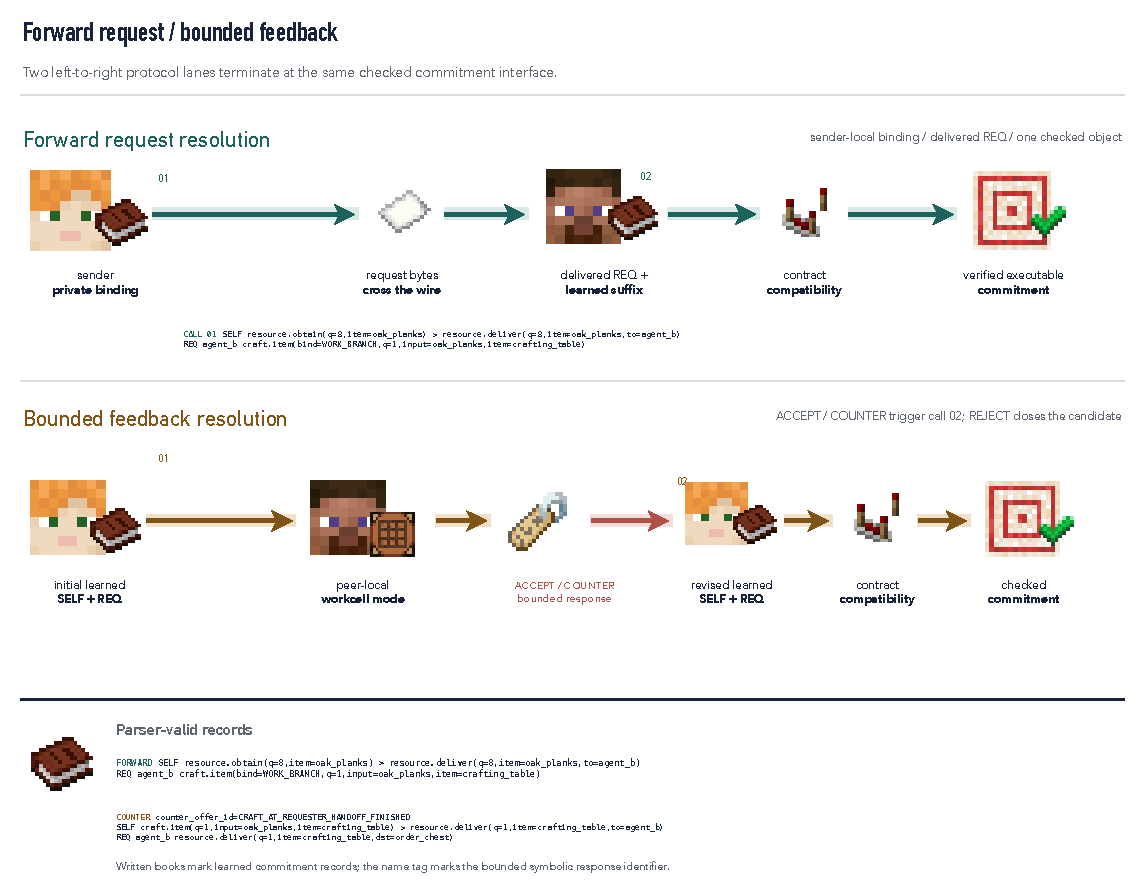
\includegraphics[width=\textwidth]{figures/figure_s2_protocol_lifecycles.pdf}
  \Description{Two Minecraft-themed execution trails show a sender-local binding moving forward in a request and a bounded workcell consequence moving backward in feedback, with learned-call counts and one checked commitment at the end of each successful trail.}
  \caption{Forward and bounded-feedback lifecycles ending in the same contract-validated commitment interface.}
  \label{fig:lifecycles}
\end{figure}

\begin{table}[!htbp]
  \centering
  \caption{Lifecycle stages and learned-call attribution. Goal--Capability uses two learned calls on the evaluated \textsc{Accept}/\textsc{Counter} branches; \textsc{Reject} terminates after the first call. For the factor backend, \artifact{active\_binding\_id} is emitted at \artifact{sender\_initial} and \artifact{accepted\_binding\_id} at \artifact{receiver\_after\_request}.}
  \label{tab:lifecycle}
  \widetabstyle
  \begin{tabularx}{\textwidth}{L{1.90cm} L{2.40cm} Z L{2.70cm} Z C{1.50cm}}
    \toprule
    \thead{Setting} & \thead{First learned output / stage} & \thead{Boundary object} & \thead{Second learned output / stage} & \thead{Deterministic / non-learned operation} & \thead{Learned calls} \\
    \midrule
    Main forward route & \artifact{sender\_initial} & delivered \artifact{REQ} & \artifact{receiver\_}\newline\artifact{after\_request} & canonical joint resolution & 2 \\
    Goal--Capability & \artifact{requester\_}\newline\artifact{initial} & bounded capability response & \artifact{requester\_}\newline\artifact{after\_response} & \artifact{ACCEPT}/\artifact{COUNTER} policy & 2 \\
    Single-step route & \artifact{sender\_initial} & request and state transition & \artifact{sender\_after\_}\newline\artifact{obtain}, then receiver & task transition & episode-\newline dependent \\
    Factor backend & \artifact{active\_}\newline\artifact{binding\_id}\newline(sender) & delivered \artifact{REQ} & \artifact{accepted\_}\newline\artifact{binding\_id}\newline(receiver) & deterministic composer & 2 \\
    \bottomrule
  \end{tabularx}
\end{table}

\begin{table}[!htbp]
  \centering
  \caption{Core notation used by Algorithms~\ref{alg:forward}--\ref{alg:feedback}.}
  \label{tab:core-notation}
  \tabstyle
  \begin{tabularx}{\textwidth}{L{3.55cm} Z}
    \toprule
    \thead{Symbol} & \thead{Meaning and domain} \\
    \midrule
    $\mathcal A=\{a_1,\ldots,a_n\}$; $i,j\in\{1,\ldots,n\}$ & agent team and indices; protocol roles are written as \emph{snd}, \emph{rcv}, \emph{req}, and \emph{peer} \\
    $\mathcal K=(\mathcal S,G,\Theta,\Gamma)$ & reusable executable prior: skill catalog $\mathcal S$, public task DAG $G$, typed schema $\Theta$, and grounding/checker contract $\Gamma$ \\
    $\xi_{\mathrm{pub}}$, $\omega_t$, $x_i^t$ & public episode instantiation, current executable world state, and agent $i$'s model-visible local context at round $t$; $\omega_t$ is visible only to the runtime verifier \\
    $\hat y_{\mathrm{snd}},q_{\mathrm{snd}}$; $\hat y_{\mathrm{rcv}},q_{\mathrm{rcv}}$ & raw model strings and parsed sender/receiver proposals; $q=\bot$ denotes parse failure \\
    $r_{\mathrm{snd}\rightarrow\mathrm{rcv}}$, $u_{\mathrm{rcv}}$ & requested peer path and receiver-local realization suffix \\
    $c_{\mathrm{peer}}$, $\rho$, $\alpha$ & peer capability, bounded response, and selected \artifact{counter\_offer\_id} \\
    $N_{\mathcal K}^{\mathrm{path}}$, $N_{\mathcal K}^{\mathrm{prop}}$, $\operatorname{Actorize}$ & canonical normalization for paths/proposals and explicit instantiation of an implicit task actor \\
    $\mathcal C$, $\mathcal D$, $\mathcal E$, $\mathcal F$ & spaces of resolved commitments, dispatch plans, no-commitment reasons, and protocol/runtime failure codes \\
    \bottomrule
  \end{tabularx}
\end{table}

The protocol result type is the tagged union
\[
\mathcal R=
(\{\mathtt{SUCCESS}\}\times\mathcal C\times\mathcal D)
\;\uplus\;
(\{\mathtt{NO\_COMMITMENT}\}\times\mathcal E)
\;\uplus\;
(\{\mathtt{FAIL}\}\times\mathcal F).
\]
We write its values as $\operatorname{Success}(C,D)$, $\operatorname{NoCommitment}(e)$, and $\operatorname{Fail}(f)$.

\begin{algorithm}[!htbp]
  \caption{Forward resolution}
  \label{alg:forward}
  \footnotesize
  \begin{algorithmic}[1]
    \Require sender context $x_{\mathrm{snd}}$, receiver context $x_{\mathrm{rcv}}$, prior $\mathcal K$, public episode instantiation $\xi_{\mathrm{pub}}$, executable world $\omega_t$
    \State $\hat y_{\mathrm{snd}} \gets \textsc{Generate}(x_{\mathrm{snd}},\mathcal K,\xi_{\mathrm{pub}})$ \Comment{\artifact{SELF+REQ}}
    \State $q_{\mathrm{snd}} \gets \textsc{Parse}(\hat y_{\mathrm{snd}})$
    \If{$q_{\mathrm{snd}}=\bot$} \State \Return $\textsc{Fail}(\mathtt{PARSE\_FAILURE})$ \EndIf
    \If{$\neg\textsc{ContractCheck}(q_{\mathrm{snd}},x_{\mathrm{snd}},\mathcal K,\xi_{\mathrm{pub}})$}
      \State \Return $\textsc{Fail}(\mathtt{CONTRACT\_REJECT})$
    \EndIf
    \If{$|q_{\mathrm{snd}}.\mathtt{peer\_requests}|\neq1$ \textbf{or} $q_{\mathrm{snd}}.\mathtt{peer\_requests}[0].\mathtt{requested\_plan}=[]$}
      \State \Return $\textsc{Fail}(\mathtt{CONTRACT\_REJECT})$
    \EndIf
    \State $r_{\mathrm{snd}\rightarrow\mathrm{rcv}}\gets q_{\mathrm{snd}}.\mathtt{peer\_requests}[0]$; deliver $r_{\mathrm{snd}\rightarrow\mathrm{rcv}}$
    \State $\hat y_{\mathrm{rcv}} \gets \textsc{Generate}(x_{\mathrm{rcv}},\mathcal K,\xi_{\mathrm{pub}},r_{\mathrm{snd}\rightarrow\mathrm{rcv}})$
    \State $q_{\mathrm{rcv}} \gets \textsc{Parse}(\hat y_{\mathrm{rcv}})$
    \If{$q_{\mathrm{rcv}}=\bot$} \State \Return $\textsc{Fail}(\mathtt{PARSE\_FAILURE})$ \EndIf
    \If{$\neg\textsc{ContractCheck}(q_{\mathrm{rcv}},x_{\mathrm{rcv}},\mathcal K,\xi_{\mathrm{pub}})$ \textbf{or} $q_{\mathrm{rcv}}.\mathtt{self\_plan}=[]$ \textbf{or} $q_{\mathrm{rcv}}.\mathtt{peer\_requests}\neq[]$}
      \State \Return $\textsc{Fail}(\mathtt{CONTRACT\_REJECT})$
    \EndIf
    \State $C \gets \textsc{Resolve}_{\rightarrow}(q_{\mathrm{snd}},q_{\mathrm{rcv}},\mathcal K,\xi_{\mathrm{pub}})$
    \If{$C=\bot$} \State \Return $\textsc{Fail}(\mathtt{RESOLUTION\_CONFLICT})$ \EndIf
    \State $D \gets \textsc{Materialize}(C,\mathcal K,\xi_{\mathrm{pub}})$
    \If{$D=\bot$} \State \Return $\textsc{Fail}(\mathtt{MATERIALIZATION\_FAILURE})$ \EndIf
    \State $\mathtt{status}\gets\textsc{ExecuteAndVerify}(D,\omega_t)$
    \If{$\mathtt{status}\neq\mathtt{SUCCESS}$} \State \Return $\textsc{Fail}(\mathtt{status})$ \EndIf
    \State \Return $\textsc{Success}(C,D)$
  \end{algorithmic}
\end{algorithm}

\begin{algorithm}[!htbp]
  \caption{Bounded feedback resolution}
  \label{alg:feedback}
  \footnotesize
  \begin{algorithmic}[1]
    \Require requester context $x_{\mathrm{req}}$, peer capability $c_{\mathrm{peer}}$, prior $\mathcal K$, public episode instantiation $\xi_{\mathrm{pub}}$, executable world $\omega_t$
    \State $\hat y_0 \gets \textsc{Generate}(x_{\mathrm{req}},\mathcal K,\xi_{\mathrm{pub}})$
    \State $q_0 \gets \textsc{Parse}(\hat y_0)$
    \If{$q_0=\bot$} \State \Return $\textsc{Fail}(\mathtt{PARSE\_FAILURE})$ \EndIf
    \If{$\neg\textsc{ContractCheck}(q_0,x_{\mathrm{req}},\mathcal K,\xi_{\mathrm{pub}})$}
      \State \Return $\textsc{Fail}(\mathtt{CONTRACT\_REJECT})$
    \EndIf
    \If{$|q_0.\mathtt{peer\_requests}|\neq1$ \textbf{or} $q_0.\mathtt{peer\_requests}[0].\mathtt{requested\_plan}=[]$}
      \State \Return $\textsc{Fail}(\mathtt{CONTRACT\_REJECT})$
    \EndIf
    \State $r_{\mathrm{req}\rightarrow\mathrm{peer}}\gets q_0.\mathtt{peer\_requests}[0]$
    \State $\rho \gets \textsc{ResponsePolicy}(r_{\mathrm{req}\rightarrow\mathrm{peer}},c_{\mathrm{peer}},\mathcal K,\xi_{\mathrm{pub}})$
    \If{$\neg\textsc{ResponseValid}(\rho,r_{\mathrm{req}\rightarrow\mathrm{peer}},\mathcal K,\xi_{\mathrm{pub}})$}
      \State \Return $\textsc{Fail}(\mathtt{CONTRACT\_REJECT})$
    \EndIf
    \If{$\rho=\textsc{Reject}$}
      \State \Return $\textsc{NoCommitment}(\rho.\mathtt{reason\_code})$
    \EndIf
    \State $\hat y_1 \gets \textsc{Generate}(x_{\mathrm{req}},\mathcal K,\xi_{\mathrm{pub}},q_0,\rho)$ \Comment{ACCEPT or COUNTER}
    \State $q_1 \gets \textsc{Parse}(\hat y_1)$
    \If{$q_1=\bot$} \State \Return $\textsc{Fail}(\mathtt{PARSE\_FAILURE})$ \EndIf
    \If{$\neg\textsc{ContractCheck}(q_1,x_{\mathrm{req}},\mathcal K,\xi_{\mathrm{pub}})$}
      \State \Return $\textsc{Fail}(\mathtt{CONTRACT\_REJECT})$
    \EndIf
    \If{$|q_1.\mathtt{peer\_requests}|\neq1$ \textbf{or} $q_1.\mathtt{peer\_requests}[0].\mathtt{requested\_plan}=[]$}
      \State \Return $\textsc{Fail}(\mathtt{CONTRACT\_REJECT})$
    \EndIf
    \If{$q_1.\mathtt{peer\_requests}[0].\mathtt{target}\neq r_{\mathrm{req}\rightarrow\mathrm{peer}}.\mathtt{target}$}
      \State \Return $\textsc{Fail}(\mathtt{CONTRACT\_REJECT})$
    \EndIf
    \State $C \gets \textsc{Resolve}_{\leftarrow}(q_0,q_1,\rho,\mathcal K,\xi_{\mathrm{pub}})$
    \If{$C=\bot$} \State \Return $\textsc{Fail}(\mathtt{RESOLUTION\_CONFLICT})$ \EndIf
    \State $D \gets \textsc{Materialize}(C,\mathcal K,\xi_{\mathrm{pub}})$
    \If{$D=\bot$} \State \Return $\textsc{Fail}(\mathtt{MATERIALIZATION\_FAILURE})$ \EndIf
    \State $\mathtt{status}\gets\textsc{ExecuteAndVerify}(D,\omega_t)$
    \If{$\mathtt{status}\neq\mathtt{SUCCESS}$} \State \Return $\textsc{Fail}(\mathtt{status})$ \EndIf
    \State \Return $\textsc{Success}(C,D)$
  \end{algorithmic}
\end{algorithm}
\FloatBarrier

The response policy selects among admissible alternatives from the grounded skill hierarchy. A response is $\rho\in\{\textsc{Accept},\textsc{Reject},\textsc{Counter}(\alpha)\}$. The bounded alternative $\alpha$ is serialized in the E1/E2 artifact as \artifact{counter\_offer\_id}; its observed counter value is \artifact{CRAFT\_AT\_REQUESTER\_HANDOFF\_FINISHED}. \artifact{ACCEPT} retains the proposed branch without an alternative, \artifact{COUNTER} names exactly one admissible alternative, and \artifact{REJECT} closes the candidate without a second generation or dispatch. Accepted and countered proposals both condition a second requester call. The transparent policy contributes zero learned calls and exposes the bounded capability consequence explicitly; Table~\ref{tab:response-schema} gives the complete response contract. The world state $\omega_t$ remains outside the model and response-policy inputs and is accessed by execution and verification.

Algorithms~\ref{alg:forward}--\ref{alg:feedback} keep parsing, contract validation, resolution, materialization, and world discharge distinct. The terminal verifier returns one of \artifact{SUCCESS}, \artifact{EXECUTION\_FAILURE}, \artifact{HANDOFF\_FAILURE}, or \artifact{TERMINAL\_FAILURE}; earlier stages return the failure codes shown in the algorithms.

\begin{table}[!htbp]
  \centering
  \caption{Finite response schema and stage-local failure codes.}
  \label{tab:response-schema}
  \tabstyle
  \begin{tabularx}{\textwidth}{L{2.45cm} Z Z}
    \toprule
    \thead{Decision / stage} & \thead{Valid fields or condition} & \thead{Protocol consequence} \\
    \midrule
    \textsc{Accept} & reason code; no \artifact{counter\_offer\_id} & second requester call preserves the normalized initial branch \\
    $\textsc{Counter}(\alpha)$ & reason code and exactly one admissible \artifact{counter\_offer\_id}=$\alpha$ & second requester call realizes the selected bounded branch \\
    \textsc{Reject} & reason code; no counter alternative & candidate closes; no second generation, commitment, or dispatch \\
    Invalid response & unknown decision, forbidden field, missing alternative, or inadmissible ID & \artifact{CONTRACT\_REJECT} \\
    \midrule
    Parse & raw string cannot be decoded & \artifact{PARSE\_FAILURE} \\
    Contract & schema, role, skill, argument, target, or response check fails & \artifact{CONTRACT\_REJECT} \\
    Resolution & realization, boundary fields, branch, or dependency merge conflicts & \artifact{RESOLUTION\_CONFLICT} \\
    Materialization & validated commitment cannot instantiate a dispatch & \artifact{MATERIALIZATION\_FAILURE} \\
    World discharge & runtime action, inventory handoff, or terminal predicate fails & \artifact{EXECUTION\_FAILURE}, \artifact{HANDOFF\_FAILURE}, or \artifact{TERMINAL\_FAILURE} \\
    \bottomrule
  \end{tabularx}
\end{table}

\subsection{Resolver semantics}

As in the main paper, a grounded task is $\tau=(a,k,\mathbf v,\ell,P)$: actor $a$, skill identifier $k$, typed arguments $\mathbf v$, grounding location $\ell$, and predecessor set $P$. A resolved commitment has the common operational form
\[
C=(S_i,S_j,b,P_C)\in\mathcal C,
\]
where $S_i$ and $S_j$ are the two normalized role-local paths, $b$ is the selected binding identifier from the public codebook, and $P_C$ is the merged predecessor relation. Protocol-specific proposals, responses, and realization records remain in the trace; $C$ contains only the operative obligations that enter materialization.

The function $\operatorname{Actorize}(z,a)$ instantiates every implicit actor in path $z$ as $a$. We use $N_{\mathcal K}^{\mathrm{path}}$ for canonical path normalization and $N_{\mathcal K}^{\mathrm{prop}}$ for proposal normalization; both canonicalize aliases, typed defaults, grounded references, bindings, actors, and predecessor semantics.

\paragraph{Forward resolution.}
Define
\[
S_{\mathrm{snd}}=N_{\mathcal K}^{\mathrm{path}}\!\left(\operatorname{Actorize}(q_{\mathrm{snd}}.\mathtt{self\_plan},\mathrm{snd})\right),
\]
\[
R_{\mathrm{rcv}}=N_{\mathcal K}^{\mathrm{path}}\!\left(\operatorname{Actorize}(r_{\mathrm{snd}\rightarrow\mathrm{rcv}}.\mathtt{requested\_plan},\mathrm{rcv})\right),
\quad
U_{\mathrm{rcv}}=N_{\mathcal K}^{\mathrm{path}}\!\left(\operatorname{Actorize}(q_{\mathrm{rcv}}.\mathtt{self\_plan},\mathrm{rcv})\right).
\]
Within the evaluated canonical contract, the receiver realizes the request exactly when
\begin{equation}
\operatorname{Realizes}_{\mathcal K}(U_{\mathrm{rcv}},R_{\mathrm{rcv}})
\iff U_{\mathrm{rcv}}=R_{\mathrm{rcv}}.
\label{eq:realizes}
\end{equation}
This equality preserves ordered task count, skills, typed values, bindings, actors, locations, and dependency semantics after normalization. Textual argument order and accepted aliases may differ. Canonical realization contains exactly the requested model-owned tasks; deterministic executor bookkeeping is added after resolution.

Let $\operatorname{HandoffCompatible}_{\mathcal K,\xi_{\mathrm{pub}}}(S_i,S_j)$ denote compatibility of the producing/receiving actors, item, quantity, source/destination references, and boundary dependency under the public episode instantiation. $\textsc{Resolve}_{\rightarrow}$ returns
\[
C^{\rightarrow}=(S_{\mathrm{snd}},U_{\mathrm{rcv}},b,P_C)
\]
only when (i) the receiver identity equals the request target; (ii) $q_{\mathrm{rcv}}$ has a nonempty \artifact{SELF} suffix and no outbound request; (iii) Equation~\ref{eq:realizes} holds; (iv) $\operatorname{HandoffCompatible}_{\mathcal K,\xi_{\mathrm{pub}}}(S_{\mathrm{snd}},U_{\mathrm{rcv}})$ holds; and (v) $b$ yields a complete acyclic predecessor merge $P_C$. The merge preserves each role-local order, retains public predecessors on the selected branch, and adds a cross-agent dependency from the contract-validated handoff producer to the first consuming receiver node. The handoff becomes \emph{verified} only after execution. Missing fields, incompatible handoffs, multiple selected branches, or cycles yield $\bot$.

\paragraph{Feedback resolution.}
Let $\mathcal B_{\mathcal K}$ be the public branch set, $B:\mathcal Q_{\mathrm{legal}}\rightarrow\mathcal B_{\mathcal K}\cup\{\bot\}$ extract the normalized branch selected by a proposal, and $\operatorname{AltBranch}_{\mathcal K,\xi_{\mathrm{pub}}}:\mathcal I_{\mathrm{alt}}\rightarrow\mathcal B_{\mathcal K}\cup\{\bot\}$ map an admissible alternative identifier to its unique branch. The response-conditioned branch is
\[
B_{\mathcal K,\xi_{\mathrm{pub}}}^{\mathrm{resp}}(\rho,q_0)=
\begin{cases}
B(q_0), & \rho=\textsc{Accept},\\
\operatorname{AltBranch}_{\mathcal K,\xi_{\mathrm{pub}}}(\alpha), & \rho=\textsc{Counter}(\alpha),\\
\bot, & \rho=\textsc{Reject}.
\end{cases}
\]
For \textsc{Accept}, the second record may use accepted surface variants while preserving the normalized operative branch, target peer, and requester goal fields of $q_0$. For $\textsc{Counter}(\alpha)$, $q_1$ preserves the requester goal fields and target peer, replaces the initial branch with the selected alternative, and realizes that branch in its operative peer request. $\textsc{Reject}$ closes the candidate after the first call.

For accepted and countered proposals, define
\[
S_{\mathrm{req}}=N_{\mathcal K}^{\mathrm{path}}\!\left(\operatorname{Actorize}(q_1.\mathtt{self\_plan},\mathrm{req})\right),
\]
\[
R_{\mathrm{peer}}=N_{\mathcal K}^{\mathrm{path}}\!\left(\operatorname{Actorize}(q_1.\mathtt{peer\_requests}[0].\mathtt{requested\_plan},\mathrm{peer})\right).
\]
The response itself is the peer-side resolution record, and the route proceeds directly to requester revision. $\textsc{Resolve}_{\leftarrow}$ requires
\[
B(q_1)=B_{\mathcal K,\xi_{\mathrm{pub}}}^{\mathrm{resp}}(\rho,q_0),
\]
$\operatorname{HandoffCompatible}_{\mathcal K,\xi_{\mathrm{pub}}}(S_{\mathrm{req}},R_{\mathrm{peer}})$, and a complete acyclic merge $P_C$, then returns
\[
C^{\leftarrow}=(S_{\mathrm{req}},R_{\mathrm{peer}},b,P_C).
\]
The protocol trace retains $q_0$ and $\rho$ as provenance, while $C^{\leftarrow}$ contains only the resolved operative paths. The materializer constructs
\[
D=\textsc{Materialize}(C,\mathcal K,\xi_{\mathrm{pub}}).
\]
It preserves the complete high-level obligation set while instantiating validated actors, locations, task-instance identifiers, dependencies, and checker attachments. The compiler then adds deterministic navigation, inventory-transfer mechanics, timeouts, claims, and runtime metadata required to realize $D$ as Mineflayer calls.

\section{Task Suite and Programmatic Supervision}
\label{sec:supp-data}

\takeaway{Four forward-request task families place the path-determining binding in the sender's local view; the delivered request disambiguates the receiver's two admissible branches.}

Table~\ref{tab:task-inventory} enumerates the eight templates and the commitment field changed by each balanced binding. Table~\ref{tab:supervision} then shows how every template produces reciprocal sender-proposal and receiver-realization supervision.

\begin{table}[!htbp]
  \centering
  \caption{Complete inventory of the eight core task templates and the commitment field varied by each binding.}
  \label{tab:task-inventory}
  \widetabstyle
  \setlength{\tabcolsep}{2.0pt}
  \begin{tabularx}{\textwidth}{L{1.65cm} L{2.15cm} L{1.75cm} Z L{2.90cm} L{1.95cm}}
    \toprule
    \thead{Family} & \thead{Template} & \thead{Source material} & \thead{Balanced bindings} & \thead{Binding-dependent request path} & \thead{Changed field} \\
    \midrule
    Destination & Build Site A/B & oak planks & \artifact{SITE\_A}/\artifact{SITE\_B} & \artifact{build.component} & destination \\
    Destination & Chest A/B & cobblestone & \artifact{CHEST\_A}/\artifact{CHEST\_B} & \artifact{resource.deliver} & destination \\
    Recipe & Chest/Crafting Table & oak planks & \artifact{CHEST}/\newline\artifact{CRAFTING\_TABLE} & \artifact{craft.item} & transform;\newline handoff item \\
    Recipe & Planks/Sticks & oak planks & \artifact{PLANKS}/\newline\artifact{STICKS} & \artifact{craft.item}/\newline\artifact{resource.deliver} & transform;\newline handoff item \\
    Allocation & Deposit/Build & cobblestone & \artifact{BUILD}/\artifact{DEPOSIT} & \artifact{build.component}/\newline\artifact{resource.deliver} & actor and remaining work \\
    Allocation & Dual Build & oak planks & \artifact{ROOF}/\artifact{WALL} & \artifact{build.component} & actor and component \\
    Active branch & Active Order & oak planks & \artifact{STORAGE}/\artifact{WORK} & \artifact{craft.item} & downstream continuation \\
    Active branch & Remaining Terminal & oak planks & \artifact{DEPOT}/\newline\artifact{MARKER} & \artifact{build.component}/\newline\artifact{resource.deliver} & downstream continuation \\
    \bottomrule
  \end{tabularx}
\end{table}

Each template has two equally represented admissible bindings. The active binding appears in the sender-local private field and is absent from the receiver-local view. Paired binding worlds keep the receiver's decision context matched until the request arrives, so removing the delivered request leaves the receiver unable to distinguish the two executable branches and produces the constructive 50\% ceiling. Every instance requires a verified material handoff and a binding-specific terminal world-state predicate.

\begin{table}[!htbp]
  \centering
  \caption{Programmatic supervision records for the forward route.}
  \label{tab:supervision}
  \tabstyle
  \begin{tabularx}{\textwidth}{L{2.3cm} Z R{1.0cm}}
    \toprule
    \thead{Record stage} & \thead{Target object} & \thead{Rows} \\
    \midrule
    Sender proposal & multi-step \artifact{SELF} plus peer \artifact{REQ} & 960 \\
    Receiver after request & downstream \artifact{SELF}; empty \artifact{REQ} & 960 \\
    Intermediate sender (single-step) & next local action after obtain & 960 \\
    \bottomrule
  \end{tabularx}
\end{table}

Targets are instantiated from task-template specifications, sampled local facts, and canonical task objects. Public Minecraft resources support ontology and scenario design; the reciprocal targets come from the executable template contract. The data builder writes the model-visible context and target separately, then validates that each target maps back to the intended binding and terminal predicate.

\section{Training and Checkpoint Provenance}
\label{sec:supp-training}

\takeaway{The checkpoint inventory makes stage coverage and optimization budget explicit. Multi-step training uses 1,920 rows and 240 updates per seed, while single-step receives an additional intermediate stage, 2,880 rows, and 360 updates.}

Tables~\ref{tab:training-budgets} and~\ref{tab:training-provenance} report the matched model configuration, stage counts, update budgets, data hashes, and checkpoint identities.

\begin{table}[!htbp]
  \centering
  \caption{Training budgets and stage coverage per random seed.}
  \label{tab:training-budgets}
  \widetabstyle
  \begin{tabularx}{\textwidth}{L{2.8cm} R{1.1cm} Z C{1.15cm} R{1.25cm} C{0.95cm}}
    \toprule
    \thead{Model or condition} & \thead{Rows} & \thead{Stage counts} & \thead{Epochs} & \thead{Steps} & \thead{Seeds} \\
    \midrule
    Multi-step / direct / surface & 1,920 & 960 sender + 960 receiver & 2 & 240 & 3 \\
    Self-plan-only & 1,920 & 960 sender + 960 receiver & 2 & 240 & 3 \\
    Matched-SFT free-form & 2,400 & 1,200 sender + 1,200 receiver & 2 & 300 & 3 \\
    Single-step & 2,880 & 960 sender + 960 intermediate sender + 960 receiver & 2 & 360 & 3 \\
    Factor backend & 1,920 & 960 sender code + 960 receiver code & 2 & 240 & 3 \\
    \bottomrule
  \end{tabularx}
\end{table}

\begin{table}[!htbp]
  \centering
  \caption{Shared training configuration and horizon-model provenance.}
  \label{tab:training-provenance}
  \widetabstyle
  \begin{tabularx}{\textwidth}{L{3.0cm} Z Z}
    \toprule
    \thead{Field} & \thead{Multi-step} & \thead{Single-step} \\
    \midrule
    \multicolumn{3}{@{}l}{\textbf{(a) Common configuration}} \\
    Base model & \multicolumn{2}{l}{Qwen3.5-0.8B \cite{qwenteam2026qwen35}; tree \artifact{1ba0a4ab\ldots}} \\
    Optimizer & \multicolumn{2}{l}{AdamW; LR $10^{-5}$; weight decay 0.01; cosine schedule; warm-up 0.03; grad-norm 1.0} \\
    Batch / precision & \multicolumn{2}{l}{micro 4; accumulation 4; effective 16; bfloat16 on A100 40GB} \\
    Length / decoding & \multicolumn{2}{l}{maximum 2,048; deterministic decoding; structured cap 256 tokens} \\
    Objective / selection & \multicolumn{2}{l}{target-and-EOS causal loss; final-step checkpoint; DEV reserved for implementation checks} \\
    \midrule
    \multicolumn{3}{@{}l}{\textbf{(b) Model-specific data and checkpoint identity}} \\
    Training rows / updates & 1,920 / 240 & 2,880 / 360 \\
    Training-data SHA-256 prefix & \artifact{f31ba0b5} & \artifact{8bdbf220} \\
    Config SHA-256 prefix & \artifact{d965b3e7} & \artifact{d965b3e7} \\
    Seed IDs & \artifact{2026073101--03} & \artifact{2026073101--03} \\
    Final checkpoint prefixes & \artifact{66e1f8c0}, \artifact{4b99b075}, \artifact{48df1656} & \artifact{9c0bd589}, \artifact{f82d702f}, \artifact{42705cf5} \\
    \bottomrule
  \end{tabularx}
\end{table}

The project-side training record stores the complete data-manifest hash, configuration hash, base-model tree hash, seed, runtime versions, token exposure, checkpoint identity, and final checkpoint tree hash. The public arXiv artifact retains the scientific configuration and content hashes while removing host, scheduler, process, and private-path identifiers.

\section{Commitment Schema and Grounded Runtime}
\label{sec:supp-runtime}

\takeaway{The model emits a compact symbolic commitment. A typed checker validates its semantics, a canonical materializer instantiates the dispatch plan, and the compiler lowers that plan to Mineflayer skills.}

\subsection{Short DSL grammar}

\begin{lstlisting}[style=gcpdsl]
program   ::= self_line NEWLINE req_line
self_line ::= "SELF -" | "SELF " path
req_line  ::= "REQ -" | "REQ " agent " " path
path      ::= task (" > " task){0,4}
task      ::= skill "(" [args] ")"
args      ::= arg ("," arg)*
arg       ::= key "=" value
key       ::= ident
value     ::= json_string | json_number
            | "true" | "false" | "null" | atom
skill     ::= control.wait | resource.obtain
            | resource.deliver | craft.item
            | transform.supply_input
            | transform.supply_fuel
            | transform.collect_output
            | build.component
ident     ::= [A-Za-z][A-Za-z0-9_]*
agent     ::= atom
atom      ::= [A-Za-z0-9_.:/+-]+
json_number ::= JSON numeric literal
json_string ::= RFC 8259 double-quoted string
\end{lstlisting}

The displayed BNF defines the canonical serializer output. Value recognition follows the displayed priority: a leading double quote starts a JSON string; a complete JSON number is recognized next; the three reserved literals precede the unquoted atom fallback. A quoted string is scanned atomically, so escaped quotes, commas, parentheses, and backslashes inside it do not terminate an argument or task. Standard JSON escapes are decoded before type checking, and unquoted atoms remain restricted to the ASCII class shown above. The canonical serializer emits exactly two LF-separated lines with normalized ASCII spacing and no leading or trailing whitespace; parser-tolerated noncanonical whitespace is outside the serializer invariant.

The serializer emits the compact keys \artifact{q}, \artifact{item}, \artifact{input}, \artifact{to}, \artifact{dst}, \artifact{bind}, \artifact{site}, \artifact{from}, \artifact{dst\_role}, \artifact{loc}, and \artifact{station}. The parser also accepts their expanded compatibility names, including \artifact{count}/\artifact{quantity}, \artifact{target\_agent\_ref}/\artifact{to\_agent\_id}, \artifact{destination}, \artifact{destination\_role}, \artifact{from\_agent\_id}, \artifact{location\_ref}, and \artifact{binding\_id}, then canonicalizes them before checking. Syntactic parsing accepts identifier-shaped keys and primitive JSON values; the skill-specific contract checker rejects unknown keys, invalid types, unknown agents, inadmissible bindings, and missing required fields. The codec rejects duplicate keys, paths outside the evaluated catalog, invalid atoms, trailing text, and an empty requested plan.

The parser requires exactly two lines and permits one to five ordered tasks per nonempty path. Quantities are positive integers; \artifact{to} names a peer; \artifact{dst}, \artifact{site}, \artifact{loc}, and \artifact{station} identify grounding references; \artifact{bind} selects an admissible branch from the public codebook. The separator \artifact{>} encodes commitment precedence; compilation expands the validated path into low-level action calls. \artifact{REQ -} is a legal record whose parsed \artifact{peer\_requests} value is the empty list; $\bot$ is reserved for parse failure, while contract rejection is represented separately by \artifact{CONTRACT\_REJECT}.

Let $\mathcal Y_{\mathrm{parse}}$ be syntactically admissible strings, $\mathcal Q_{\mathrm{parsed}}$ parsed proposal objects, and $\mathcal Q_{\mathrm{legal}}(\mathcal K,\xi_{\mathrm{pub}})$ the subset satisfying the typed contract. Define
\[
\operatorname{Parse}:\mathcal Y_{\mathrm{parse}}\rightarrow\mathcal Q_{\mathrm{parsed}}\cup\{\bot\},
\qquad
\operatorname{ContractCheck}_{\mathcal K,\xi_{\mathrm{pub}}}:\mathcal Q_{\mathrm{parsed}}\rightarrow\{\mathtt{true},\mathtt{false}\}.
\]
The legal-string domain is
\[
\mathcal Y_{\mathrm{legal}}(\mathcal K,\xi_{\mathrm{pub}})
=
\left\{y\in\mathcal Y_{\mathrm{parse}}:\operatorname{Parse}(y)\neq\bot,\;
\operatorname{ContractCheck}_{\mathcal K,\xi_{\mathrm{pub}}}(\operatorname{Parse}(y))=\mathtt{true}\right\}.
\]
Let $\mathcal Y_{\mathrm{canon}}(\mathcal K)$ be canonical serializer outputs. For legal strings, the semantic decoder and encoder are
\[
\operatorname{Decode}_{\mathcal K,\xi_{\mathrm{pub}}}(y)
=
N_{\mathcal K}^{\mathrm{prop}}\!\left(\operatorname{Parse}(y)\right),
\quad y\in\mathcal Y_{\mathrm{legal}}(\mathcal K,\xi_{\mathrm{pub}}),
\]
\[
\operatorname{Encode}_{\mathcal K}:\mathcal Q_{\mathrm{legal}}(\mathcal K,\xi_{\mathrm{pub}})\rightarrow\mathcal Y_{\mathrm{canon}}(\mathcal K).
\]
For legal DSL strings $y_1,y_2$,
\begin{equation}
y_1\equiv_{\mathrm{sem}}y_2
\iff
\operatorname{Decode}_{\mathcal K,\xi_{\mathrm{pub}}}(y_1)
=
\operatorname{Decode}_{\mathcal K,\xi_{\mathrm{pub}}}(y_2).
\end{equation}
For $Q\in\mathcal Q_{\mathrm{legal}}(\mathcal K,\xi_{\mathrm{pub}})$, the tested codec invariant is
\begin{equation}
\operatorname{Decode}_{\mathcal K,\xi_{\mathrm{pub}}}(\operatorname{Encode}_{\mathcal K}(Q))
=
N_{\mathcal K}^{\mathrm{prop}}(Q).
\end{equation}
The invariant is defined and verified over the fixed schema, evaluated task families, and shared executable prior used in this study. Within that contract, the decoded object retains the ordered self path, target peer, ordered requested path, typed arguments, bindings, actors, grounding references, and dependency semantics required to determine the resolved route.

\begin{lstlisting}[style=gcpdsl]
SELF resource.obtain(q=8,item=oak_planks) >
     resource.deliver(q=8,item=oak_planks,to=agent_a)
REQ agent_a craft.item(bind=WORK_BRANCH,q=1,
     input=oak_planks,item=crafting_table)
\end{lstlisting}

Table~\ref{tab:contract-checks} separates the checks that establish a valid commitment from the post-materialization and post-execution evidence that discharges it.

\begin{table}[!htbp]
  \centering
  \caption{Checks across parsing, materialization, and live verification.}
  \label{tab:contract-checks}
  \tabstyle
  \begin{tabularx}{\columnwidth}{L{2.35cm} L{2.25cm} Z}
    \toprule
    \thead{Phase} & \thead{Check} & \thead{Accepted condition} \\
    \midrule
    Pre-materialization & Syntax and identity & two-line grammar; actors and peer match the role instance \\
     & Skill and arguments & catalog path, required keys, types, and quantities are valid \\
     & Binding and handoff & branch is admissible; item, quantity, sender, and receiver agree \\
     & Dependency merge & selected predecessor graph is complete and acyclic \\
    Post-materialization & Static plan consistency & resolved actors, fields, handoff edge, and checker attachment match the validated commitment \\
    Post-execution & World verification & handoff event and declared terminal predicate both pass \\
    \bottomrule
  \end{tabularx}
\end{table}

The live route is
\begin{align*}
\text{generate}&\rightarrow\text{parse}\rightarrow\text{contract check}\\[-2pt]
&\rightarrow\text{canonical materialize}\rightarrow\text{compile}\\[-2pt]
&\rightarrow\text{execute}\rightarrow\text{verify}.
\end{align*}
Once the model-generated semantics equal the selected canonical task object, the materializer combines the selected binding with the shared task structure. Mineflayer~4.37.1 \cite{prismarinejs2026mineflayer} then executes the compiled skills against the official Minecraft Java server~1.21.4.

Figure~\ref{fig:runtime-trace} follows one retained episode from learned records to terminal world state; Table~\ref{tab:runtime-accounting} reports the exact calls, actions, inventory deltas, and wall-clock time for the same trace.

\begin{figure}[!htbp]
  \centering
  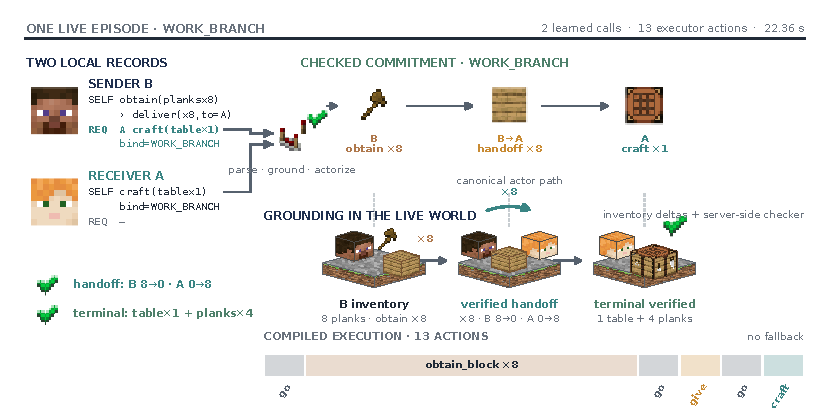
\includegraphics[width=\textwidth]{figures/figure_s3_grounded_runtime_trace.pdf}
  \Description{Two local Short DSL records merge into one checked actorized commitment. The compiled execution obtains eight oak planks, transfers them from Agent B to Agent A, and reaches the verified terminal inventory containing one crafting table and four remaining planks.}
  \caption{One grounded episode from bilateral Short DSL records to a checked commitment, verified handoff, and terminal world state.}
  \label{fig:runtime-trace}
\end{figure}

\begin{table}[!htbp]
  \centering
  \caption{Representative live episode accounting.}
  \label{tab:runtime-accounting}
  \tabstyle
  \begin{tabularx}{\textwidth}{Z R{2.30cm}}
    \toprule
    \thead{Event or state} & \thead{Observed value} \\
    \midrule
    Selected binding & \artifact{WORK\_BRANCH} \\
    Learned model calls & 2 \\
    Executor actions & 13 \\
    Sender oak planks, before $\rightarrow$ after & $8\rightarrow0$ \\
    Receiver oak planks, before $\rightarrow$ after & $0\rightarrow8$ \\
    Terminal crafting tables & 1 \\
    Wall-clock episode time & 22.36 s \\
    Handoff / terminal verification & pass / pass \\
    \bottomrule
  \end{tabularx}
\end{table}

Figure~\ref{fig:runtime-trace} uses role instance \apath{GCP-PAPER-REP-ACTIVE-ORDER-BRANCH-0015-R1}. The trace records inventory snapshots around the handoff, all issued skills, the terminal inventory, and the server-side checker result.

\section{Full Quality and Communication Results}
\label{sec:supp-quality}

\takeaway{At matched terminal quality, the three communication surfaces differ sharply in generated length, message size, and time-to-commitment while sharing the same executor.}

Table~\ref{tab:representation-results} establishes the quality lock and reports the exact online costs. Figure~\ref{fig:cost-fingerprint} makes the resulting cost profile visually comparable, and Table~\ref{tab:reliability-latency} separates same-card call latency from quality-pool reliability.

\begin{table}[!htbp]
  \centering
  \caption{Matched-quality representation results. Success uses the 128-cluster quality pool; calls, token counts, protocol-specific Agent-to-Agent payload bytes, and TTC use the separate 40-cluster same-card timing pool.}
  \label{tab:representation-results}
  \widetabstyle
  \begin{tabularx}{\textwidth}{Z R{1.2cm} R{0.8cm} R{1.15cm} R{1.15cm} R{1.1cm} R{1.15cm} R{1.15cm}}
    \toprule
    \thead{Method} & \thead{Success} & \thead{Calls} & \thead{Input tok.} & \thead{Output tok.} & \thead{Wire B} & \thead{TTC p50} & \thead{TTC p95} \\
    \midrule
    \dsl GenCoord (0.8B) & 100.0\% & 2.0 & 949.1 & 78.6 & 76.3 & 2.266 s & 2.616 s \\
    JSON GenCoord (0.8B) & 100.0\% & 2.0 & 1,154.7 & 267.6 & 303.4 & 7.067 s & 7.864 s \\
    Controlled free-form + structured commit (0.8B) & 100.0\% & 2.5 & 1,585.2 & 265.8 & 1,061.1 & 7.132 s & 7.857 s \\
    \bottomrule
  \end{tabularx}
\end{table}

\begin{figure}[!htbp]
  \centering
  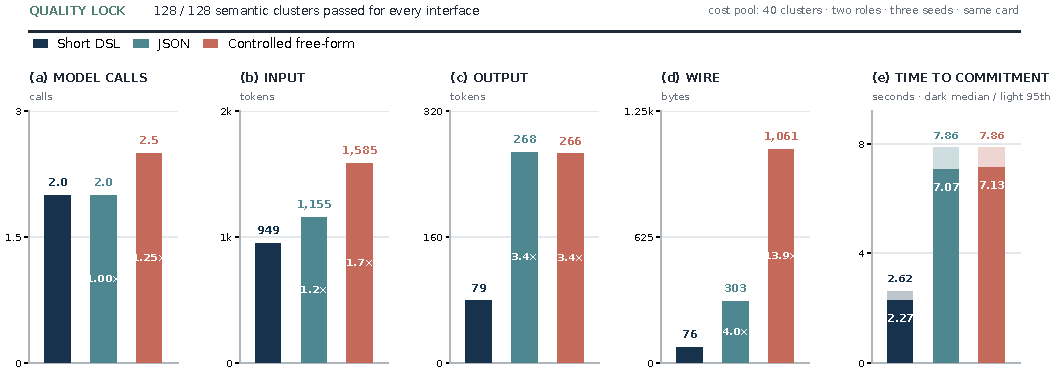
\includegraphics[width=\textwidth]{figures/figure_s4_coordination_cost_fingerprint.pdf}
  \Description{Five aligned bar panels compare model calls, input tokens, output tokens, Agent-to-Agent wire bytes, and same-card time-to-commitment for three interfaces that all pass the 128-cluster quality pool. In the TTC panel, the dark bar ends at p50, the median, and the pale extension ends at p95, the 95th percentile.}
  \caption{Quality-matched coordination costs on independent physical-unit axes. All three interfaces pass the 128-cluster quality pool; costs use the separate 40-cluster same-card timing pool. In the TTC panel, dark bars end at p50 (the median) and pale extensions end at p95 (the 95th percentile).}
  \label{fig:cost-fingerprint}
\end{figure}

\begin{table}[!htbp]
  \centering
  \caption{Same-card latency and quality-pool reliability. The two panels retain their separate 40- and 128-cluster denominators.}
  \label{tab:reliability-latency}
  \tabstyle
  \begin{tabularx}{\columnwidth}{Z R{1.25cm} R{1.25cm}}
    \toprule
    \multicolumn{3}{@{}l}{\textbf{(a) Call latency: 40-cluster same-card pool}} \\
    \thead{Surface} & \thead{p50} & \thead{p95} \\
    \midrule
    \dsl call latency & 1.143 s & 1.660 s \\
    JSON call latency & 3.531 s & 5.941 s \\
    Controlled free-form call latency & 3.274 s & 3.746 s \\
    \midrule
    \multicolumn{3}{@{}l}{\textbf{(b) Reliability and symmetry: 128-cluster quality pool}} \\
    Strict successful clusters, each surface & \multicolumn{2}{r}{128/128} \\
    Exact-binomial 95\% lower bound & \multicolumn{2}{r}{0.972} \\
    Role-swap success difference & \multicolumn{2}{r}{0.0 pp} \\
    Missing / fallback rows & \multicolumn{2}{r}{0 / 0} \\
    \bottomrule
  \end{tabularx}
\end{table}

The same-card timing pool contains 40 clusters, two role views, and three checkpoints per surface. Models run sequentially on the same device. TTC ends when the executable bilateral commitment is available; executor time begins after commitment and remains near 22.6 s p50 across surfaces.

\section{Request Semantics and Strong Baselines}
\label{sec:supp-request}

\takeaway{The delivered binding is causally active: removing it restores the paired 50\% ceiling, while replacing it with the other executable option drives the receiver to the paired world-state branch.}

Table~\ref{tab:request-intervention} holds message presence, protocol schedule, schema, and learned-call count fixed while changing only the delivered task content; the deterministic row supplies an exact binding-selection ceiling for the enumerable library.

\begin{table}[!htbp]
  \centering
  \caption{Request intervention and deterministic binding reference on 160 clusters. Learned rows contain three seeds (960 episodes); the seedless deterministic rule runs once per role view (320 episodes). Paired differences are true request minus the listed condition. Bytes are canonical request-object JSON, distinct from the protocol-specific Short DSL request-line bytes in Table~\ref{tab:representation-results}.}
  \label{tab:request-intervention}
  \widetabstyle
  \begin{tabularx}{\textwidth}{L{2.7cm} R{1.45cm} R{1.25cm} R{0.9cm} R{1.1cm} R{1.45cm} Z}
    \toprule
    \thead{Condition} & \thead{Episodes} & \thead{Success} & \thead{Calls} & \thead{Req.-object JSON B} & \thead{True $-$ condition} & \thead{Mechanism readout} \\
    \midrule
    True learned request & 960 & 100.0\% & 2.0 & 304.4 & 0.0 pp & reference success \\
    Request removed / self-plan-only & 960 & 50.0\% & 2.0 & 0.0 & $+50.0$ pp $[42.5,57.5]$ & paired ambiguity exposed \\
    Same-template executable alternative & 960 & 0.0\% & 2.0 & 304.4 & $+100.0$ pp $[100,100]$ & receiver follows delivered alternative \\
    Deterministic correct binding & 320 & 100.0\% & 0.0 & 304.4 & $0.0$ pp & exact binding ceiling \\
    \bottomrule
  \end{tabularx}
\end{table}

The alternative intervention selects the other executable request from the same template option set and preserves message presence, schedule, schema, approximate length, and learned-call count. The receiver follows the delivered alternative in 960/960 CONFIRM episodes and 471/471 executable held-out cases. Every executable held-out output preserves the delivered binding; the nine residual losses occur before an executable plan is formed.


\section{Commitment Horizon and Template Shift}
\label{sec:supp-horizon}

\takeaway{Under the corresponding closed-loop training protocols, multi-step commitments improve held-out success and reduce online decisions; the gain concentrates in allocation and active-continuation templates.}

Table~\ref{tab:horizon} reports the paired aggregate effects and family decomposition; Figure~\ref{fig:horizon-family} shows where the success gain appears and how much online burden remains.

\begin{table}[!htbp]
  \centering
  \caption{Held-out-template horizon results across 80 independent clusters. Every difference is multi-step minus single-step. Family rows are descriptive; confidence intervals are reported for the aggregate paired comparisons.}
  \label{tab:horizon}
  \widetabstyle
  \begin{tabularx}{0.995\textwidth}{L{2.25cm} R{1.2cm} R{1.2cm} R{1.15cm} L{2.35cm} Z}
    \toprule
    \thead{Family / metric} & \thead{Multi-step} & \thead{Single-step} & \thead{$\Delta$} & \thead{95\% CI} & \thead{Interpretive feature} \\
    \midrule
    Destination & 100.0\% & 100.0\% & 0.0 pp & \textemdash{} & destination binding \\
    Recipe & 100.0\% & 100.0\% & 0.0 pp & \textemdash{} & transformation binding \\
    Allocation & 92.5\% & 83.3\% & 9.2 pp & \textemdash{} & actor / remaining workload \\
    Active branch & 100.0\% & 81.7\% & 18.3 pp & \textemdash{} & downstream continuation \\
    \midrule
    Overall success & 98.1\% & 91.3\% & 6.9 pp & $[2.9,10.8]$ pp & paired cluster bootstrap \\
    Decisions / episode & 1.981 & 2.913 & $-0.931$ calls / ep. & $[-0.971,-0.892]$ calls / ep. & online coordination cost \\
    Input tokens / episode & 1,146.5 & 1,689.1 & $-542.6$ tok./ep. & $[-567.8,-517.6]$ tok./ep. & repeated context avoided \\
    \bottomrule
  \end{tabularx}
\end{table}

\begin{figure}[!htbp]
  \centering
  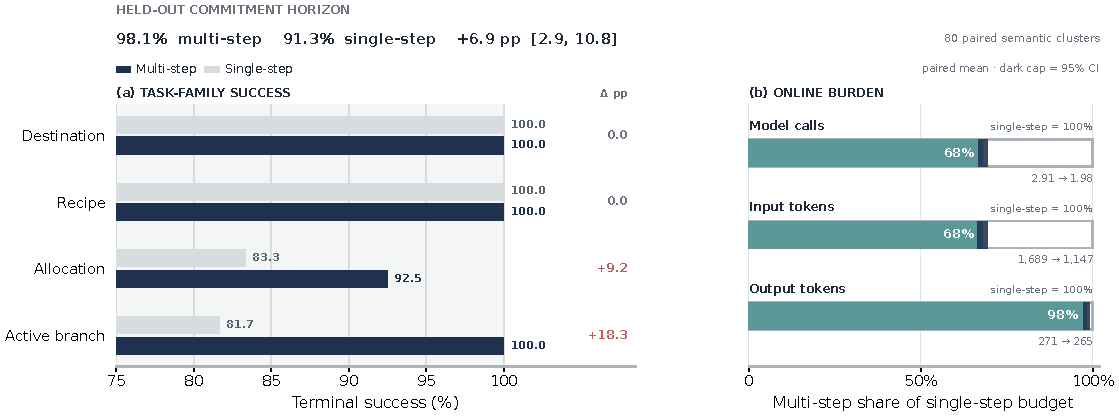
\includegraphics[width=\textwidth]{figures/figure_s5_horizon_family_effects.pdf}
  \Description{Panel a uses paired horizontal bars to compare multi-step and single-step terminal success within each task family and reports their percentage-point difference. Panel b represents single-step as a full 100-percent budget outline and fills the share consumed by multi-step for model calls, input tokens, and output tokens; the dark cap maps the paired absolute-difference interval to the observed single-step denominator.}
  \caption{Paired commitment-horizon comparison over 80 held-out semantic clusters. (a) Task-family terminal success. (b) Multi-step online burden as a share of the corresponding single-step mean; dark caps map the paired absolute-difference confidence intervals from Table~\ref{tab:horizon} onto that observed denominator.}
  \label{fig:horizon-family}
\end{figure}

The comparison evaluates complete systems under their corresponding training protocol. Multi-step training uses 1,920 rows and 240 optimizer updates per seed. Single-step training uses 2,880 rows, 360 updates, and an additional \artifact{sender\_after\_obtain} stage. This design gives the single-step system explicit intermediate-state supervision; the measured difference therefore combines commitment horizon with each protocol's online control pattern.

The deterministic correct-binding rule supplies an exact binding-selection ceiling on the same held-out pool: 100.0\% versus 98.1\% for multi-step GenCoord, a paired GenCoord-minus-rule difference of $-1.9$ pp (95\% CI $[-4.2,-0.2]$). GenCoord preserves the correct binding in every executable output; its nine residual losses arise before plan formation. The comparison therefore separates exact binding sufficiency from learned commitment formation while retaining the same executable interface.

\section{Backend and Composition Analyses}
\label{sec:supp-backend}

\takeaway{For the enumerable task library, a learned binding code plus deterministic rule is a faster quality-matched backend. Direct Short DSL retains an explicit executable path as its model output.}

Table~\ref{tab:backend} isolates backend formation while holding the peer-facing commitment fixed. Table~\ref{tab:factor-minimality} then separates complete-case lookup from field-wise construction on unseen binding cross-products.

\begin{table}[!htbp]
  \centering
  \caption{Quality-matched direct and factor-code backends. Fresh success uses 128 clusters (two roles, three seeds); token counts and TTC use a separate 40-cluster same-card planning pool.}
  \label{tab:backend}
  \tabstyle
  \begin{tabularx}{\columnwidth}{Z R{1.55cm} R{1.55cm}}
    \toprule
    \thead{Metric} & \thead{Factor + rule} & \thead{Direct DSL} \\
    \midrule
    Fresh success & 768/768 & 768/768 \\
    Input tokens & 980.2 & 948.9 \\
    Output tokens & 19.4 & 79.1 \\
    Protocol-specific peer payload & 76.6 B & 76.6 B \\
    TTC p50 & 0.824 s & 2.453 s \\
    TTC p95 & 0.997 s & 2.723 s \\
    \bottomrule
  \end{tabularx}
\end{table}

The factor target is the sender binding ID before delivery and the receiver accepted-binding ID after delivery. Both models receive the same model-visible information. A deterministic composer recovers actor, path, object, destination, dependencies, and the same peer-facing Short DSL request from the selected code.

\begin{table}[!htbp]
  \centering
  \caption{Composition reference on 60 unseen binding cross-products.}
  \label{tab:factor-minimality}
  \tabstyle
  \begin{tabularx}{\textwidth}{Z R{2.30cm}}
    \toprule
    \thead{Method} & \thead{Terminal success} \\
    \midrule
    Complete-case table & 0/60 \\
    Explicit-factor composer & 60/60 \\
    Direct Short DSL & 60/60 \\
    \bottomrule
  \end{tabularx}
\end{table}

The composition reference separates exact case lookup from field-wise construction. Explicit factor composition and Direct Short DSL recover all 60 tested cross-products, while exact complete-case lookup covers the observed cases only. Table~\ref{tab:backend} further shows that, when a public codebook uniquely determines the branch, factor-code generation provides a lower-latency path to the same peer-facing commitment.

\subsection{Naturalized private facts without binding IDs}

The active binding field is next replaced by naturalized private-fact descriptions while the same 16 semantic task cells, public prior, and grounded executor are retained. Table~\ref{tab:naturalized-private} reports one Minecraft closed-loop condition with test-only syntactic recombinations and two stronger planning-only surface shifts.

\begin{table}[!htbp]
  \centering
  \caption{Naturalized private-fact formation after removing the active binding field. C1 is Minecraft closed-loop evaluation on held-out syntactic recombinations; C2 and C3 are planning-only lexical-paraphrase and paraphrase-plus-distractor conditions. Learned rows aggregate three seeds (960 episodes per condition); seedless model-free rows use 320 episodes.}
  \label{tab:naturalized-private}
  \tabstyle
  \begin{tabularx}{\textwidth}{Z R{2.15cm} R{2.15cm} R{2.15cm}}
    \toprule
    \thead{Formation method} & \thead{C1 live} & \thead{C2 planning} & \thead{C3 planning} \\
    \midrule
    Direct Short DSL (0.8B) & 100.0\% & 65.8\% & 64.8\% \\
    Learned factor + rule (0.8B) & 100.0\% & \textbf{79.1\%} & \textbf{80.1\%} \\
    Frozen factor parser rule & 100.0\% & 0.0\% & 0.0\% \\
    TF--IDF nearest-neighbour rule & 100.0\% & 59.4\% & 62.5\% \\
    Complete surface table & 0.0\% & 0.0\% & 0.0\% \\
    Oracle factors + rule & 100.0\% & 100.0\% & 100.0\% \\
    \bottomrule
  \end{tabularx}
\end{table}

Under C1, both learned backends and the two stronger non-LLM semantic mappings retain 100\% closed-loop success, while exact-string lookup covers the training surfaces only. The commitment interface therefore remains executable after the active answer field is replaced by test-only naturalized descriptions. Under stronger surface shifts, learned factor formation reaches 79.1\% and 80.1\%, exceeding TF--IDF by $+19.7$ pp (95\% CI $[11.8,27.9]$) and $+17.6$ pp ($[9.2,26.5]$), respectively; Direct Short DSL reaches 65.8\% and 64.8\%. The result strengthens the interface/backend separation: compact factor prediction is the more robust realization under stronger lexical change.

\section{Task-Structure Visibility}
\label{sec:supp-visibility}

\takeaway{Full and Skeleton views preserve the familiar post-handoff branch; the analysis cleanly separates that recovered motif from transformation-order motifs that require additional structural generalization.}

Figure~\ref{fig:visibility} reports the full 3-method $\times$ 3-view $\times$ 3-motif matrix with exact percentages in every cell.


\begin{figure}[!htbp]
  \centering
  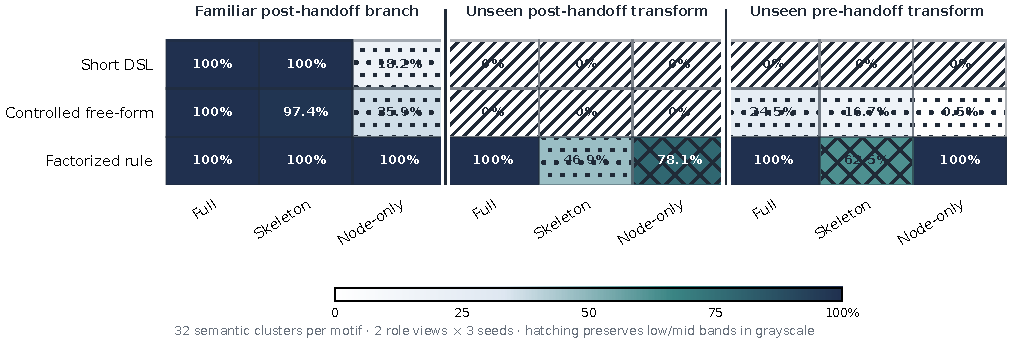
\includegraphics[width=\textwidth]{figures/figure_s6_visibility_motif_fingerprint.pdf}
  \Description{A three-by-nine annotated heatmap reports exact success percentages for three methods, three public-structure projections, and three topology motifs; cell outlines and labels remain distinguishable in grayscale.}
  \caption{Annotated task-structure robustness matrix. Columns pair each topology motif with Full, Skeleton, and Node-only projections; cells show exact terminal success.}
  \label{fig:visibility}
\end{figure}

Full DAG exposes the public nodes, typed fields, coarse stages, predecessor lists, and edges; its symbolic reference follows a topological ordering. Skeleton removes predecessor lists and edges while retaining coarse stage, and its symbolic reference uses that stage information. Node-only removes stages and edges, applies a stable answer-independent node arrangement, and uses a fixed task-path priority. The three views are categorical projections with distinct answer-independent ordering policies. Across 96 clusters, two role views, and three frozen checkpoints, the matrix shows that Direct Short DSL preserves the familiar post-handoff branch under Full and Skeleton views, while the two transformation-order motifs remain at 0\%. The symbolic rule's non-monotone Node-only recovery reflects its fixed task-path priority under a different projection.

\section{E1/E2: Feedback Causality and Centralized Reference}
\label{sec:supp-private}

\takeaway{Across 40 Goal--Capability semantic clusters (20 matched counterfactual pairs) and three independently trained seeds, requester-local planning reaches 50\%, correct feedback reaches 100\%, counterfactual feedback reaches 0\%, and centralized full information reaches 100\%.}

\subsection{Paired construction and matched training}

The evaluation crosses two private goals, two peer-local workcell modes, and ten world variants, producing $2\times2\times10=40$ semantic clusters. Table~\ref{tab:e1e2-training} records the matched training contracts; Table~\ref{tab:private-info} reports the four-condition outcome profile; Table~\ref{tab:e1-field-fidelity} isolates the fields controlled by feedback; and Figure~\ref{fig:private-traces} traces the capability-conditioned routes and intervention. Holding goal and world variant fixed while changing the workcell mode creates 20 matched counterfactual pairs. Within each pair, the requester's model-visible input and initial proposal are byte-identical; the peer-local mode changes the feasible craft actor, handoff object, and downstream suffix. Each condition evaluates all 40 clusters under two role permutations and three training seeds, yielding 240 episodes per condition and 960 episodes overall. The primary analysis averages the six role--seed observations within semantic cluster and resamples 40 clusters. A pair-block sensitivity analysis additionally averages both capability worlds within each goal--world pair and resamples the 20 matched pair blocks.

\begin{table}[!htbp]
  \centering
  \caption{Training contracts for the Goal--Capability models. Train-token occurrences sum tokenized prompt, target, and EOS across all epochs.}
  \label{tab:e1e2-training}
  \tabstyle
  \begin{tabularx}{\textwidth}{@{}Z Z r r r r r@{}}
  \toprule
  \thead{Model} & \thead{Visible information} & \thead{Rows} & \thead{Epochs} & \thead{Updates} & \thead{Train-token occurrences} & \thead{Seeds} \\
  \midrule
  Distributed requester & 320 initial local + 320 after-response local & 640 & 2 & 80 & 868,720 & 3 \\
  Centralized full information & merged current local views & 320 & 4 & 80 & 970,080 & 3 \\
  \bottomrule
\end{tabularx}

\end{table}

The distributed data contain 320 initial local records and 320 local records after the bounded response. The centralized data contain 320 joint-plan records. Both models use Qwen3.5-0.8B, effective batch size 16, learning rate $10^{-5}$, maximum length 2,048, and final-step checkpoints, with DEV reserved for implementation checks. Matching optimizer updates gives the centralized model 1.117 times the distributed train-token occurrences. The reported totals include prompt, target, and EOS tokens over all sample occurrences; every row remains below the 2,048-token truncation limit.

\subsection{E1: feedback-content intervention}

\begin{table}[!htbp]
  \centering
  \caption{E1/E2 outcomes on 40 semantic clusters, arranged as 20 matched counterfactual pairs. Intervals are primary cluster-bootstrap 95\% CIs. Strict success requires all six role--seed observations of a cluster to succeed; the final column names the measured boundary component rather than total architecture traffic.}
  \label{tab:private-info}
  \tabstyle
  \begin{tabularx}{\textwidth}{@{}Z r r r c r r Z@{}}
  \toprule
  \thead{Condition} & \thead{Seeds} & \thead{Epis.} & \thead{Success} & \thead{95\% CI} & \thead{Strict} & \thead{Calls} & \thead{Measured boundary component} \\
  \midrule
  Requester-local (A-only) & 3 & 240 & 50.0\% & $[35,65]$ & 20/40 & 1.0 & 0 B cross-boundary payload \\
  Correct bounded feedback & 3 & 240 & 100.0\% & $[100,100]$ & 40/40 & 2.0 & response: mean 103 B \\
  Counterfactual feedback & 3 & 240 & 0.0\% & $[0,0]$ & 0/40 & 2.0 & injected response: mean 103 B \\
  Centralized full information & 3 & 240 & 100.0\% & $[100,100]$ & 40/40 & 1.0 & state aggregation: mean 956 B \\
  \bottomrule
\end{tabularx}

\end{table}

Correct feedback improves success over requester-local planning by $+50.0$ percentage points (primary 40-cluster 95\% CI $[35,65]$). Replacing only the response with the paired counterfactual workcell mode changes the same two-call protocol from 100\% to 0\% (paired difference $+100.0$ points, 95\% CI $[100,100]$). The 20-pair block sensitivity gives $+50.0$ points $[50,50]$ and $+100.0$ points $[100,100]$, respectively. Every seed reproduces the 50/100/0 profile with descriptive seed-level SD 0.0. All 720 distributed episodes are parse-valid, condition-specific contract-valid, planning-complete, and fallback-free. Counterfactual commitments remain internally valid under the injected response, while the unchanged executable world provides an independent terminal check.

\begin{table}[!htbp]
  \centering
  \caption{Commitment fields under the counterfactual-feedback intervention.}
  \label{tab:e1-field-fidelity}
  \tabstyle
  \begin{tabularx}{\textwidth}{@{}Z r r Z@{}}
  \toprule
  \thead{Field} & \thead{Matches injected} & \thead{Matches true world} & \thead{Observed behavior} \\
  \midrule
  Craft actor & 240/240 & 0/240 & rewritten \\
  Handoff item & 240/240 & 0/240 & rewritten \\
  Handoff count & 240/240 & 0/240 & rewritten \\
  Peer suffix & 240/240 & 0/240 & rewritten \\
  Goal item & 240/240 & 240/240 & invariant \\
  Goal count & 240/240 & 240/240 & invariant \\
  \bottomrule
\end{tabularx}

\end{table}

The intervention preserves the requester input, initial proposal, executable world, model checkpoints, decoding contract, and two-call schedule. Counterfactual feedback controls the final commitment in all 240 episodes: craft actor, handoff item, handoff count, and peer suffix follow the injected capability consequence, while goal item and goal count remain unchanged. Each complete commitment therefore reaches the actor selected by the injected response, and the unchanged world rejects that counterfactual actor at terminal verification.

\begin{figure}[!htbp]
  \centering
  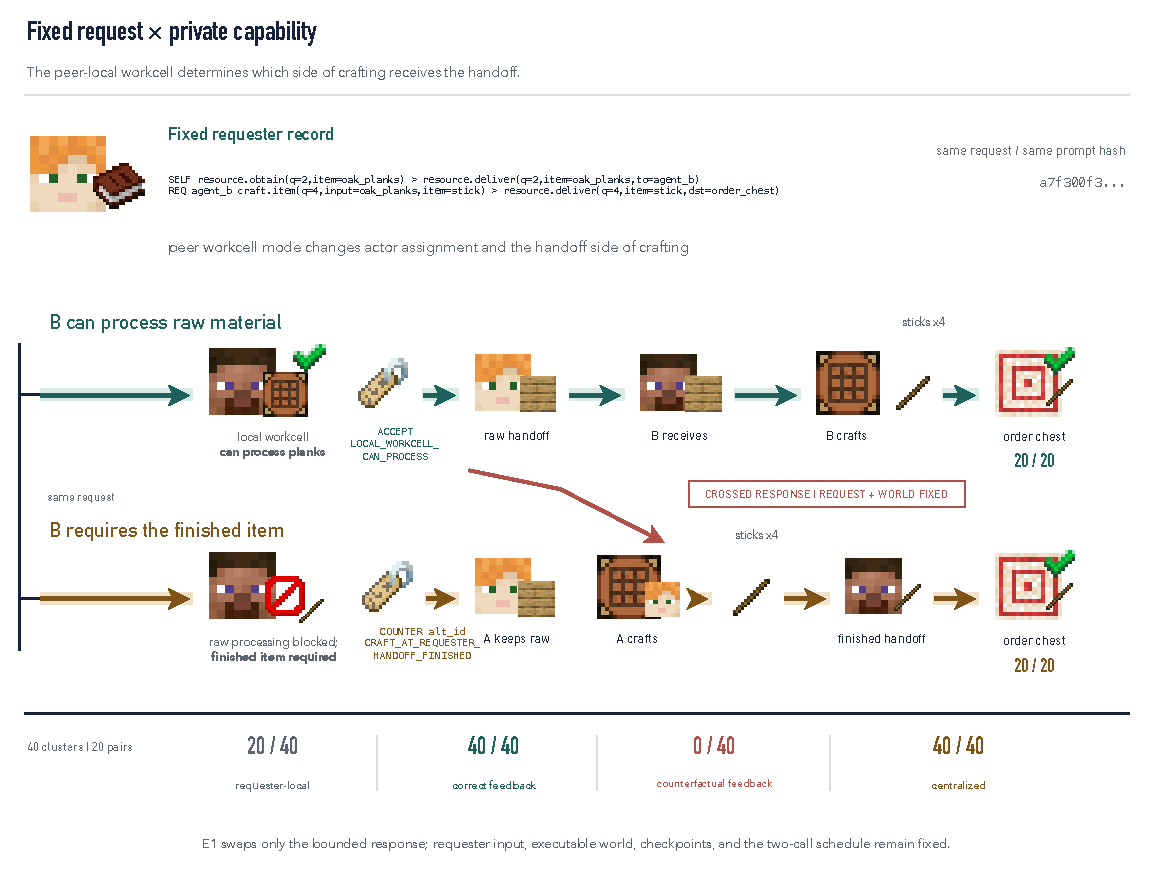
\includegraphics[width=\textwidth]{figures/figure_s7_goal_capability_counterfactuals.pdf}
  \Description{A requester record and its prompt hash remain fixed above a capability fork; the peer fact routes execution through accepted raw-material or countered finished-item handoff paths, while a counterfactual-feedback intervention keeps the requester and executable world fixed.}
  \caption{Capability-conditioned commitments and the counterfactual-feedback intervention with requester input and executable world held fixed.}
  \label{fig:private-traces}
\end{figure}

Figure~\ref{fig:private-traces} illustrates a correct-feedback pair that shares one requester prompt hash. A \apath{RAW_PROCESSOR} peer accepts the raw-material handoff. A \apath{FINISHED_RECEIVER} peer counters with \apath{CRAFT_AT_REQUESTER_HANDOFF_FINISHED}; the requester moves crafting into its own path and hands off the finished item. Both correct routes reach the terminal checker. The E1 intervention injects the matched counterfactual response while keeping the requester input, initial proposal, and executable world fixed.

\subsection{E2: three-seed centralized reference}

Centralized full information succeeds in 240/240 episodes across the same three seeds and 40 clusters, matching correct feedback with a paired difference of 0.0 points (95\% CI $[0,0]$). It assembles the two current local views before one learned call. The distributed route keeps the views separate and uses a bounded response with mean 103 B and p95 118 B before its second learned call. The centralized state-aggregation component has mean 955.5 B and p95 963 B (rounded to 956 B in Table~\ref{tab:private-info}). The 103 B value measures the bounded response, while 955.5 B measures centralized state aggregation. The architecture-level equations below account for every application message and make the component boundaries explicit.

\Needspace{12\baselineskip}
\begin{samepage}
For architecture accounting, let $\mathcal A_t\subseteq\mathcal A$ be the participating agents at round $t$, let $E_t\subseteq\mathcal A\times\mathcal A$ be the directed active-edge set, and let $\mathcal M_{ij}^t$ be the complete sequence of application messages sent on directed edge $(i,j)$. The function $b(m)$ counts canonical UTF-8 payload bytes, including any application wrapper present in $m$ but excluding transport framing. Let $m_{i,\uparrow}^{t}$ and $m_{i,\downarrow}^{t}$ denote centralized upload and download payloads. With $R_c$ centralized rounds and $R_l$ local rounds,
\begin{align}
B_{\mathrm{central}}
  &= \sum_{t=1}^{R_c}\sum_{i\in\mathcal A_t}
     \left[b(m_{i,\uparrow}^{t})+b(m_{i,\downarrow}^{t})\right], \\
B_{\mathrm{local}}
  &= \sum_{t=1}^{R_l}\sum_{(i,j)\in E_t}
     \sum_{m\in\mathcal M_{ij}^{t}} b(m).
\end{align}
Feedback sent in the reverse direction belongs to the corresponding edge $(j,i)$. These equations define total interface accounting and are distinct from the component measurements above. Both architectures depend on coordination rounds; local communication also depends on active-edge density and messages per active edge.
\end{samepage}

\section{Reproducibility Notes}
\label{sec:supp-artifact}

Pre-release validation checks the bundled compact data, method identities, pool denominators, non-null horizon means, paired-difference direction, confidence intervals, bootstrap seeds, and 10,000 resamples. It also checks the corrected single-step inventory of 2,880 rows, three stage counts of 960, and 360 optimizer updates per seed. For E1/E2, the arXiv ancillary data contain twelve evaluation lanes and 960 episode metrics stripped of host, scheduler, process, and private-path identifiers, including all 240 counterfactual-feedback control episodes. The deterministic table builder regenerates Tables~\ref{tab:e1e2-training}--\ref{tab:e1-field-fidelity} from the canonical analysis and matched training-budget files. Earlier representation, request, horizon, and visibility results are reconstructed from the bundled aggregate analyses and fixed paired-comparison records; E1/E2 additionally include de-identified episode-level metrics.

\paragraph{Statistical procedure.}
Representation, request, horizon, visibility, and the primary E1/E2 analyses use the semantic cluster as the independent unit. Where role views or training seeds repeat a cluster, their outcomes are averaged within cluster before inference. Paired effects use cluster-aligned differences. Reported bootstrap intervals use 10,000 percentile resamples with fixed analysis seeds; E1/E2 condition intervals use seeds 8901--8904 and primary paired-difference intervals use 8911--8914. The E1/E2 sensitivity aggregates both capability clusters within each goal--world pair and resamples 20 pair blocks with seeds 8921--8924. Exact-binomial intervals are two-sided 95\% Clopper--Pearson intervals. Seed-level standard deviations summarize training-run stability, while cluster bootstrap intervals provide inferential uncertainty.


Table~\ref{tab:claim-artifact-map} links every reader-facing result family to its compact canonical source.

\begin{table}[!htbp]
  \centering
  \caption{Claim-to-artifact map for the compact arXiv ancillary bundle.}
  \label{tab:claim-artifact-map}
  \tabstyle
  \begin{tabularx}{\textwidth}{L{3.0cm} Z}
    \toprule
    \thead{Result family} & \thead{Canonical bundle artifact} \\
    \midrule
    Evidence-suite and task inventory & \apath{anc/source_data/evidence_suites.csv}; \apath{anc/source_data/task_templates.csv} \\
    Representation quality and cost & \apath{anc/source_data/representation_cost.csv} \\
    Request intervention & \apath{anc/source_data/request_intervention.csv} \\
    Commitment horizon & \apath{anc/source_data/horizon_summary.json}; \apath{anc/source_data/horizon_family.csv}; \apath{anc/source_data/paired_comparisons.json} \\
    Structure visibility & \apath{anc/source_data/visibility_motifs.csv}; \apath{anc/source_data/visibility_overall.csv} \\
    Grounded runtime trace & \apath{anc/source_data/runtime_trace.json}; \apath{anc/source_data/trace_registry.csv} \\
    E1/E2 outcomes and field fidelity & \apath{anc/source_data/e1e2_episode_metrics.jsonl}; \apath{anc/source_data/e1e2_analysis.json}; \apath{anc/source_data/e1e2_field_fidelity.csv}; \apath{anc/source_data/e1e2_config.json} \\
    Training budgets and runs & \apath{anc/source_data/e1e2_training_budget.json}; \apath{anc/source_data/training_runs.csv} \\
    Backend and composition references & \apath{anc/source_data/backend_comparison.csv}; \apath{anc/source_data/composition_reference.csv} \\
    Naturalized private-fact formation & \apath{anc/source_data/naturalized_private_fact_summary.csv}; \apath{anc/source_data/naturalized_private_fact_paired.csv}; \apath{anc/source_data/naturalized_private_fact_scope.json} \\
    Table regeneration & \apath{anc/scripts/build_e1e2_tables.py} \\
    \bottomrule
  \end{tabularx}
\end{table}

\noindent\begin{minipage}{\textwidth}
\paragraph{Packaged sources.}
The arXiv package contains the bibliography, canonical Supplement source, compact ancillary source data, final vector figure exports, and deterministic E1/E2 table builder. Reader-facing paths are package-relative. Experimental runtime dependencies include Qwen3.5-0.8B, Mineflayer~4.37.1, Node.js, Python, PyTorch, Transformers, and the official Minecraft Java server~1.21.4; each is governed by its upstream license or terms.
\end{minipage}

\paragraph{Build sequence.}
Regenerate the E1/E2 tables with:
\begin{lstlisting}[style=gcpdsl]
python3 anc/scripts/build_e1e2_tables.py \
  --analysis anc/source_data/e1e2_analysis.json \
  --training anc/source_data/e1e2_training_budget.json \
  --tables-dir tables --data-dir anc/source_data
\end{lstlisting}
Then compile \apath{supplement.tex} with the bundled bibliography. Final vector figure PDFs are included under \apath{figures/}; editable authoring sources, render caches, and contact sheets are intentionally excluded from the arXiv upload package.

\bibliographystyle{ACM-Reference-Format}
\bibliography{references}
\end{document}
